\section{Implementation Details}
Source code is uploaded to \url{https://github.com/mintcd/iot-mobile-app}.

\subsection{Server Hosts}
The TCP host is \url{tcp://io.adafruit.com:1883} and the WS host is \url{ws://io.adafruit.com:443}.

\subsection{Dataflows}

The IoT devices include

\begin{itemize}
  \item Two sensors of temperature and humidity. They publish environmental data to the Adafruit server's corresponding feeds. By default, the frequency is set to $5$ seconds.
  \item Two household devices, a bulb and an air-conditioner. They publish state data frequently to the corresponding feeds similarly to the sensors. Also, the bulb subscribes to \texttt{bulb-controller}, and the air-conditioner subscribes to \texttt{air-conditioner-controller} and \texttt{temperature}.
\end{itemize}

The UI client subscribes to the \texttt{temperature}, \texttt{humidity}, \texttt{bulb} and \texttt{air-conditioner} feeds.

\subsection{Logic}

\begin{figure}[ht]
  \centering
  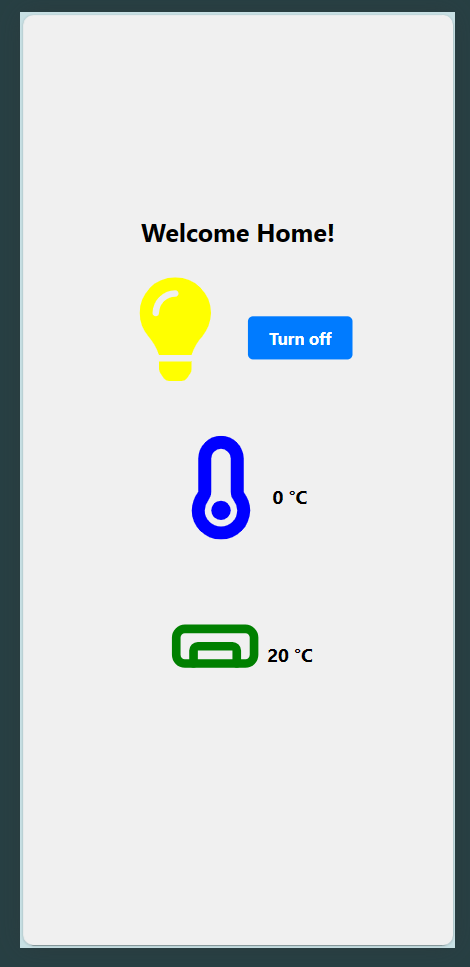
\includegraphics[width=0.5\textwidth]{img/app-ui.png}
  \vspace{0.5cm}
  \caption{The App UI}
\end{figure}

UI's received data from the subscribed feeds are rendered. Bulb and Air-conditioner fetch data from \texttt{bulb-controller} (0 or 1) and \texttt{air-conditioner-controller} (temperature value) published from UI to change their value. Air-conditioner also fetches data from \texttt{temperature} to turn on at 20 °C and turn off automatically.